%\documentclass[10pt,a4paper]{article}
\documentclass[letterpaper,10pt,draftclsnofoot,onecolumn]{article}
\usepackage[letterpaper, margin=.75in]{geometry}

\usepackage{hyperref}
\usepackage{listings}
\usepackage{wasysym}
\usepackage{graphicx}

\graphicspath{ {./images/}}

\hypersetup{
	colorlinks,
	citecolor=black,
	filecolor=black,
	linkcolor=black,
	urlcolor=black
}

\begin{document}
\begin{titlepage}
\vspace*{\fill}
\begin{center}
{\Large Tut-Tut, The IoT Rain Fall Detector Requirements Document}
\\[0.3cm]

{\large CS 461 - Fall 2018}
\\[0.3cm]

{\large Jonathan Rohr}
\\[0.3cm]

{\large Michael Gillett}
\\[0.3cm]

{\large Shreyans Khunteta}
\\[0.3cm]

{\large October 23, 2018}
\\[1cm]

{\Large Abstract}
\end{center}
Tut-Tut, the IoT Raindrop Detector, is a project under the domain of the OPEnS (Openly Published Environment Sensing) Lab at Oregon State University. Tut-Tut will be able to detect a drop of any size, get an idea of the raindrop mass from the intensity at which it falls, and detect the frequency of raindrops. After Tut-Tut gathers this data, it will be able to wirelessly transmit the information to a central server and communicate it to other IoT devices around Oregon State University. The detector will wake up with a single raindrop and will stay awake as long as rain is detected within a minute. If it does not detect raindrops within a minute, it will go back to sleep. In addition to the physical device, we will also design an online mobile application to which the physical device will transmit information about the raindrops.
\vspace*{\fill}
\end{titlepage}

\section{Introduction}
In this document we will be outlining the requirements of Tut-Tut, the Internet of Things (IoT) Rainfall Detector. Requirements are as per requested by Chet Udell and the OPEnS Lab located at Oregon State University.

\subsection{Purpose}
This document intends to guide development of Tut-Tut over the course of 7 months. It will go through changes in the duration of the project as new information makes itself clear.

\begin{enumerate}
    \item \textbf{Draft:}  The first draft is written by the development team after requirements have been outlined by their client. 
    \item \textbf{Proposal:} The drafted document will be passed along to all other parties involved, including the client, OPEnS lab team, and course professors, who will evaluate the requirements outlines and request changes where necessary.
    \item \textbf{Approved:} The document is considered approved when it is accepted by all parties. Following this, the development team can begin implementing their technology using the document as a guide.
\end{enumerate}

\subsection{Target Audience}
This product is designed to accommodate any person(s) who may want to know about rainfall metrics in their area. The sensor will provide real-time information about the size of the rain drops and how frequently they are falling. These metrics could be used by meteorologist as a way to show more detailed information about the rain in the local area. Furthermore, the Tut-Tut Rainfall Detector will link into the OPEnS lab's larger ecosystem of environmental devices and sensors, known as Loom.

\subsection{Project Scope}
%describes the expectations of the product if it were to hit the market, e.g. what must be done to deliver the working product
When the Tut-Tut is finished at the end of the development period, it will be expected to perform three major tasks and one task that will be implemented if there is time. First, it will need to be able to translate vibrations from rainfall using its on-board vibration sensors. Second, it will transmit the collected data to an internet hub where it is subsequently uploaded to Google Sheets in real-time. Third, it must be integrated into the existing OPEnS Lab's ecosystem of sensors and devices called Loom. Finally, if time permits, a browser UI will be used to communicate the Tut-Tut data in an easy to understand way.

\subsection{Business Case for the Product}
%Why do we need this product in the world?
From a business standpoint, this product could deliver an understanding of the rainfall for different areas in the form of a comprehensive map. If the Tut-Tut rainfall detector were to be placed around the country, it could tell you about the type of rain that falls in a given region. Rain on the East Coast might be more of a mist, while the rain in Oregon falls quickly and intense. Tut-Tut would give us the data to show those claims in the form of data it gathers.

\subsection{Overview}
%Summary of the requirements, a general idea
In order to create this device, we will need to program our microcontroller, test vibration sensors, design and 3D print the enclosure, store all code in a github repository, integrate it into Loom, and if possible, create a browser UI as a way to highlight useful information in the spreadsheets.

\section{General Description}
%SECTION TWO, THE REAL DEAL
%Non-technical description, easily read in laymans terms
The IoT raindrop detector will be used to record the amount of rainfall in a particular area. This can be particularly useful in agricultural farming, as this means farmers will know exactly how much rainfall their crops are getting and this way the farmers know how much rainfall they have to provide their crops. 

\subsection{Product Perspective}
%Why are we developing this product?
The thought behind this product's development is that the Loom network managed by Oregon State's OPEnS lab lacks a device that provides more specific details about rainfall. When this product is finished and integrated into their network, the findings might be significant enough to allow Tut-Tut to be available to the public. Even if the data turns out to only be significant to a small population of people, we still will have helped out those individuals, and the Loom network will have a new integration that could inspire similar devices.

\subsection{Product Functions}
%What does it do? Main functions
The main functions of this raindrop detector are that it can detect raindrop size, frequency rate and intensity. It also will link up with the network of IoT devices maintained by the OPEnS lab. It will also upload its data to a central server where the information can be viewed in an Excel document.

\subsection{End User Characteristics}
%What would someone using the final product expect from it? Who would that person be? Do they need a technical background or can they use it right away with no prior knowledge of its development?
If we develop the mobile application (which is our stretch goal), the end user can be anyone capable of using the interface. We plan to have a user-friendly interface where anyone can use the application to see the performance metrics of the IoT device.
\newline
If we don't meet the stretch goal, the end user will be anyone able to use the Loom network of IoT devices around Oregon State. This project will be then used next year for another Capstone team to build off of.

\subsection{Constraints}
%Any constraints that might get in the way of development?
One of the biggest constraints of the project is time. All the members of this team are seniors at Oregon State. This is a project we are doing on the side after our classes and jobs, so we have to cut time out of our schedules to work on it. We have created a Standards document which we have all agreed to to deal with this problem in advance.
\newline
But more than that a constraint is Professor Udell's time. He is extremely busy so if we have questions, getting a meeting can be difficult. We have set up a meeting at 10 am every Thursday to circumvent this problem as well.
\newline
Another constraint is equipment. We will be using OPEnS lab equipment for this entire project. We are also totally reliant on them for everything so if some equipment breaks or proves ineffective, we will wait for the lab to get us new equipment.
\newline
Another constraint is expertise. We're students who are doing a project of this magnitude for the first time. We will be learning a lot during this experience but there is absolutely going to be a learning curve. It will take time for us to get up to speed.

\subsection{Assumptions and Dependencies}
%Dependencies (internet connection within range, battery or plug, etc) Assumptions (End User skills or prior knowledge)
Using this product effectively will require an internet connection and a power source. The Feather M0 microcontroller comes equipped with a Wi-Fi card, so anywhere on the university should be suitable enough for Tut-Tut. Using the device anywhere else must have a Wi-Fi signal within range. Another dependency is the power source. Because Tut-Tut is intended to be moved around, Tut-Tut should run on a battery. The type of battery we will use is undetermined, and will be figured out in the testing phase. Users should need no prior knowledge to configure and set up Tut-Tut.

\section{Specific Requirements}
This section of the document lists specific requirements for Tut-Tut. Requirements will be divided into three sections:
\begin{enumerate}
    \item \textbf{User Requirements: } These are requirements written from the point of view of the end users who will be using the product.
    \item \textbf{System Requirements: } These are the detailed specifications that the product's internal hardware will need to be capable of doing.
    \item \textbf{Interface Requirements: } These are the requirements about how the information gathered by the device will be presented 
\end{enumerate}

\subsection{User Requirements}
%Minimal, since the information will be understood by everyone
The user will, provided our stretch goal is met, be anyone. The information will be easily accessible and understandable. Even if our stretch goal isn't met, we will still display our data gathered in an Excel document that should be able to be understood by anyone.

\subsection{System Requirements}
%2x2 inch sensor capable of detecting even the most minute amounts of rain, wifi or network capabilities, able to be integrated with mesh network, waterproof
The system will be a 2x2 inch waterproof sensor capable of detecting even the most minute amounts of rain. It will have wi-fi or network capabilities and we will be able to integrate it easily with the IoT mesh network around the university. It will be able to detect the size of a raindrop, the frequency at which rain is falling, and the intensity at which it hits the detector.

\subsection{Interface Requirements}
%needs to be accessible and give accurate or clear information. Perhaps in the form of a generated map visual, or a twitter bot.
The interface for the mobile application, if the stretch goal isn't met, will just be an Excel spreadsheet with all the data cleanly labelled. If the stretch goal is met, it will be a mobile application that can easily be navigated. The specifics of the application's appearance will be worked out, but it will be easy to look at and trivial for an inexperienced user to find all the information they are looking for.

\section{Gantt Chart}
%Chart outlining the timeline of this project. Term one is design, Term two is bulding, and Term 3 is testing. That's my only information


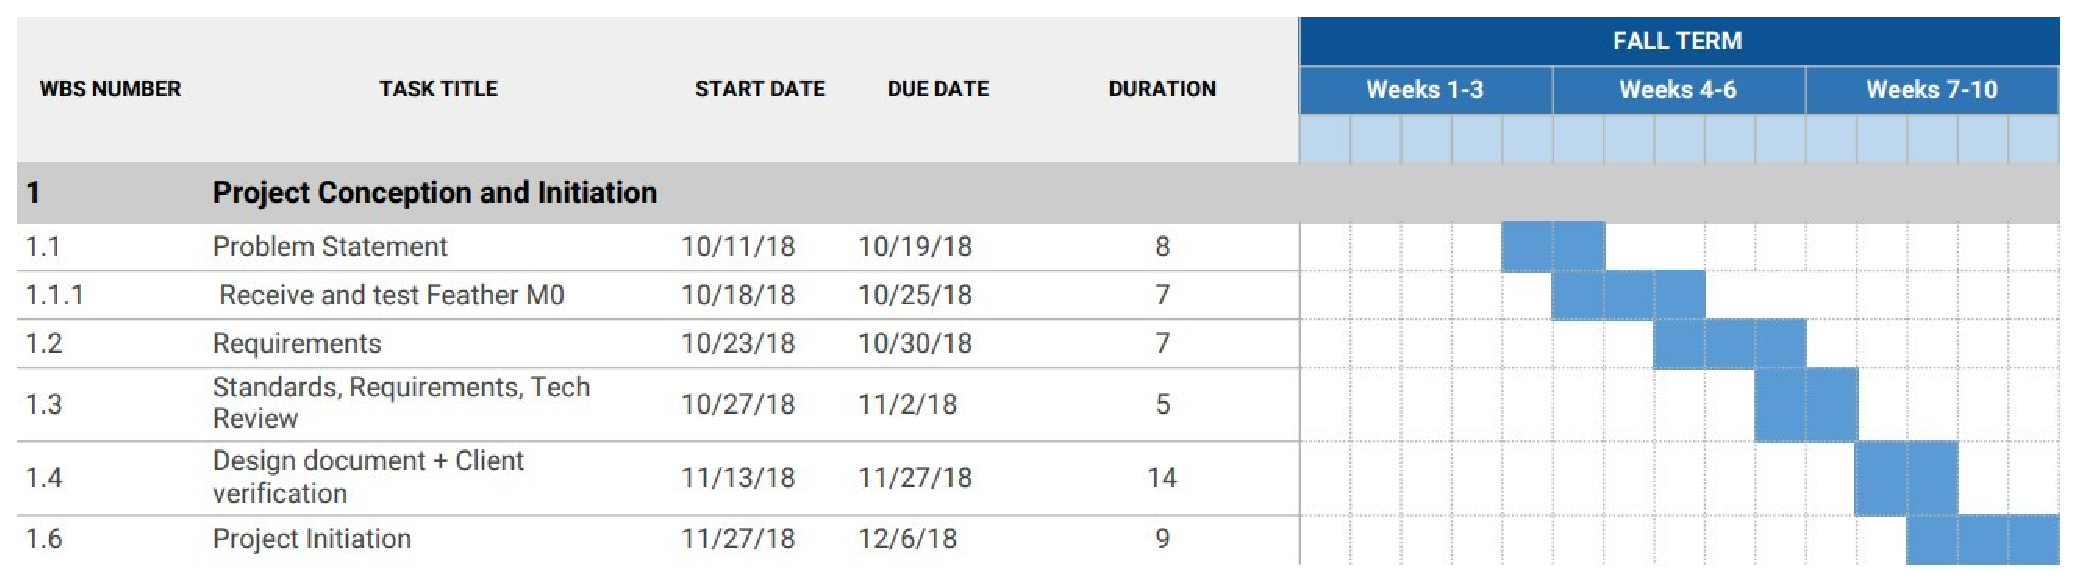
\includegraphics[scale=0.55]{GanttChart.eps}
\newline


\bibliography{myref}
\bibliographystyle{ieeetr}

\end{document}t}
